\section{Rôle d'un système d'exploitation}

% Fig Archi {{{
\begin{figure}
\centering
\begin{tikzpicture}
[ every node/.style={}
, node distance=2cm
]

\node (cpu) {CPU};

\node[below of=cpu] (northb) {Northbridge};

\node[right of=northb] (mem) {Mémoire};
\node[left of=northb]  (agp) {AGP};
\node[below of=northb] (southb) {Southbridge};

\node[below left of=southb, xshift=-1cm] (sata) {SATA};
\node[below right of=southb, xshift=1cm] (usb)  {USB};

\node[below left of=sata]  (hdd)     {Disque dur};
\node[below right of=sata] (cdrom)   {CD-ROM};

\node[below left of=usb]  (memo)    {Mémorette};
\node[below right of=usb] (clavier) {Clavier};

\draw (cpu) -- (northb);
\draw (northb) -- (agp);
\draw (northb) -- (mem);
\draw (southb) -- (northb);
\draw (southb) -- (sata);
\draw (southb) -- (usb);
\draw (usb) -- (memo);
\draw (usb) -- (clavier);
\draw (sata) -- (hdd);
\draw (sata) -- (cdrom);

\end{tikzpicture}

\caption{Architecture simplifiée d'un ordinateur}
\label{fig:archi-simplifiee}
\end{figure}
% }}}

Au plus bas, un ordinateur est constitué de nombreux composants matériels :
micro-processeur, mémoire, et divers périphériques
(figure~\ref{fig:archi-simplifiee}). Et au niveau de l'utilisateur, de dizaines
de logiciels permettant d'effectuer toutes sortes de calculs et de
communication. Le système d'exploitation permet de faire l'interface entre ces
niveaux d'abstraction. Dans ce chapitre nous allons voir son rôle et une
implantation possible. Pour une description plus détaillée, on pourra se référer
à l'ouvrage \cite{tanenbaum}.

Au cours de l'histoire des systèmes informatiques, la manière de les programmer
a beaucoup évolué. Au départ, les programmeurs avaient accès au matériel dans
son intégralité : toute la mémoire pouvait être accédé, toutes les instructions
pouvaient être utilisées.

Néanmoins c'est un peu restrictif : si on est seul à utiliser un système, on est
par définition... seul à pouvoir l'utiliser. Dans la seconde moitié des années
60, sont apparus les premiers systèmes "à temps partagé", permettant à plusieurs
utilisateurs de travailler en même temps.

Permettre l'exécution de plusieurs programmes en même temps est une idée
révolutionnaire, mais elle n'est pas sans difficultés techniques : en effet les
ressources de la machine doivent être aussi partagées entre les utilisateurs et
les programmes. Par exemple, plusieurs programmes vont par exemple utiliser le
CPU les uns à la suite des autres (partage \emph{temporel}) ; et chaque
programme aura à sa disposition une partie de la mémoire principale, ou du
disque dur (partage \emph{spatial}).

Si deux programmes (ou plus) s'exécutent de manière concurrente sur le même
matériel, il faut s'assurer par exemple que les deux s'exécutent à peu près
aussi souvent, ou que l'un ne puisse pas écrire dans la mémoire de l'autre. Ce
sont des rôles du système d'exploitation.

Cela passe donc par un certain bridage des possibilités du programme : plutôt
que de le faire exécuter n'importe quel type d'instruction, il communique avec
le système d'exploitation. Bien que cela ait l'air d'une limitation, c'est aussi
bénéfique pour le programmeur puisque cela permet de définir des abstractions au
niveau du noyau.

Par exemple, si un programmeur veut copier des données depuis un CD-ROM vers la
mémoire principale, il devra interroger le bus SATA, interroger le lecteur sur
la présence d'un disque dans le lecteur, activer le moteur, calculer le numéro
de \emph{frame} des données sur le disque, demander la lecture, puis déclencher
une copie de la mémoire.

Si dans un autre cas il voulait récupérer des données depuis une mémorette USB,
il devrait interroger le bus USB, rechercher le bon numéro de périphérique, le
bon \emph{endpoint} dans celui-ci, lui appliquer une commande de lecture au bon
numéro de bloc, puis copier la mémoire.

Ces deux opérations, bien qu'elles aient le même but (copier de la mémoire
depuis un périphérique amovible), ne sont pas effectuées en pratique de la même
manière. C'est pourquoi le système d'exploitation fournit les notions de
fichier, lecteur, etc : le programmeur n'a plus qu'à utiliser des commandes de
haut niveau (``monter un lecteur'', ``ouvrir un fichier'', ``lire dans un
fichier'') et selon le type de lecteur, le système d'exploitation effectuera les
actions appropriées.

En résumé, un système d'exploitation est l''intermédiaire entre le logiciel et
le matériel, et en particulier assure les rôles suivants :

\paragraph{Gestion des processus} : un système d'exploitation peut permettre
d'exécuter plusieurs programme à la fois. Il faut alors orchestrer ces
différents processus et les séparer en terme de temps et de ressources
partagées.

\paragraph{Gestion de la mémoire} : chaque processus, en plus du noyau, doit
disposer d'un espace mémoire différent. C'est-à-dire qu'un processus ne doit pas
pouvoir interférer avec un autre.

\paragraph{Gestion des périphériques} : le noyau étant le seul code à s'exécuter
en mode privilégié, c'est lui qui doit communiquer avec les périphériques
matériels.

\paragraph{Abstractions} : le noyau fournit au programmes une interface unifiée,
permettant de stocker des informations de la même manière sur un disque dur ou
une clef USB (alors que l'accès se déroulera de manière très différente en
pratique). C'est ici que la notion arbitraire de fichier sera définie, par
exemple.

\section{Architecture}

Dans cette section nous décrivons le fonctionnement d'un processeur utilisant
une architecture Intel 32 bits.

\subsection{Processeur}

Au coeur du processeur, se trouve une ALU (\emph{Arithmetical \& Logical Unit},
unité arithmétique et logique) qui peut réaliser des opérations comme
l'addition, la soustraction ou le "ET" logique.

Les opérandes peuvent être des registres, qui sont des petites zones de mémoire
temporaire internes au processeur, ou une adresse mémoire \footnote{C'est une
simplification : d'une part, toutes les combinaisons ne sont pas possibles, et
d'autres part, des modes d'adressages plus complexes comme "la valeur à
l'adresse égale à tel registre plus tel décalage"}.

Les registres les plus courants sont nommés \eax, \ebx, \ecx, \edx, \esi, \edi.
Ils peuvent être utilisés pour n'importe quel type d'opération, mais certains
sont spécialisés. Par exemple il est plus efficace d'utiliser \eax en
accumulateur, ou \ecx en compteur.

\esp est le pointeur de pile (\emph{stack pointer}), qui a un rôle particulier
dans les instructions \asminstr{push} et \asminstr{pop} décrites ci-dessous.

\ebp est le pointeur de trame (\emph{frame pointer}) et sert de point de repère
dans les appels de fonction. Ceci sera aussi expliqué.

\eip est l'adresse de l'instruction courante.

\eflags est un registre de "fanions" (\emph{flags}), qui sont des indicateurs
positionnés selon le résultat d'un calcul précédent.

\subsection{Assembleur}

Le processeur exécute une suite d'instructions. En voici quelques exemples.
Syntaxe AT\&T (Linux).

\begin{itemize}

\item \texttt{mov src, dest} copie le contenu de \texttt{src} dans \texttt{dst}.

\item \texttt{add src, dest} calcule la somme des contenus de \texttt{src} et
  \texttt{dst} et place ce résultat dans \texttt{dst}. Il met à jour \eflags:
  par exemple

\item \texttt{push src} place \texttt{src} sur la pile, c'est à dire que cette
  instruction décrémente le pointeur de pile \esp de la taille de \texttt{src},
  puis place \texttt{src} à l'adresse mémoire de la nouvelle valeur \esp.

\item \texttt{pop src} réalise l'opération inverse : elle charge le contenu de
  la mémoire à l'adresse \esp dans \texttt{src} puis incrémente \esp de la
  taille correspondante.

\item \texttt{jmp addr} saute à l'adresse \texttt{addr} : c'est l'équivalent de
  \texttt{mov addr, \%eip}.

\item \texttt{call addr} sert aux appels de fonction : cela revient à
  \texttt{push \%eip} puis \texttt{jmp addr}.

\item \texttt{call addr} sert à revenir d'une fonction : c'est l'équivalent de
  \texttt{pop \%eip}.

\end{itemize}

\todo{parler de modes d'adressage}

\subsection{Appel de fonction et conventions d'appel}

Au niveau de l'assembleur, il n'y a pas directement de notion de fonction ; mais
\asminstr{call} et \asminstr{ret} permettent de sauvegarder et de restaurer une
adresse de retour, ce qui permet de faire un saut et revenir à l'adresse initiale.
Ce système permet déjà de créer des procédures, c'est-à-dire des fonctions sans
arguments ni valeur de retour.

Pour gérer ceux-ci, il faut que les deux morceaux (appelant et appelé) se
mettent d'accord sur une convention d'appel commune. La convention utilisée sous
GNU/Linux est appelée \emph{cdecl} et possède les caractéristiques suivantes :

\begin{itemize}
\item la valeur de retour d'une fonction est stockée dans \eax
\item \eax, \ecx et \edx peuvent être écrasés sans avoir à les sauvegarder
\item les arguments sont placés sur la pile (et enlevés) par l'appelant. Les
  paramètres sont empilés de droite à gauche.
\end{itemize}

Pour accéder à ses paramètres, une fonction peut donc utiliser un adressage
relatif à \esp. Cela peut fonctionner, mais cela complique les choses si elle
contient aussi des variables locales. En effet, les variables locales sont
placées sur la pile, au dessus des (c'est à dire, empliées après) paramètres,
augmentant le décalage.

La solution est d'utiliser un pointeur de trame toujours égal à une position
fixe dans la pile (comme l'adresse de retour).

\begin{figure}
\begin{tikzpicture}
[ stack/.style={draw,shape=rectangle,minimum height=1cm,minimum width=5cm}
, bigbrace/.style={decorate,decoration={brace,amplitude=3mm}}
, >=latex
]

  \path (0,-8.5)   node [stack, minimum height=2cm] (gloc) {Locales de g}
  -- ++(0,1.5) node [stack] (gebp) {Cadre précédent}
  -- ++(0,1)   node [stack] (gret) {Retour de g}
  -- ++(0,1.5) node [stack, minimum height=2cm] (gpar) {Arguments de g}
  -- ++(0,1.5) node [stack] (floc) {Locales de f}
  -- ++(0,1)   node [stack] (febp) {Cadre précédent}
  -- ++(0,1)   node [stack] (fret) {Retour de f}
  -- ++(0,1)   node [stack] (fpar) {Arguments de f};

  \draw [->] (gebp) -- ++(4, 0) |- (febp.355);
  \draw [->] (febp.5) -- ++(1.5, 0) -- ++(0,4);

  \draw [dashed] (fpar.north west) -- ++ (0,2);
  \draw [dashed] (fpar.north east) -- ++ (0,2);
  \draw [dashed] (gloc.south east) -- ++ (0,-2);
  \draw [dashed] (gloc.south west) -- ++ (0,-2);

  \node at (5, 1) (ox) {};

  \node [text width=3cm] at (-0.8, 2)     {Adresses hautes (sens de \asminstr{pop})};
  \node [text width=3cm] at (-0.8, -10.5) {Adresses basses (sens de \asminstr{push})};

  \node [text width=3cm] at (-6, -3) (asmtext) {\tt
    call f\\
    ... \\
    f:  ... \\
    pushl \$2 \\
    pushl \$4 \\
    call g \\
    addl \$8, \%esp \\
    leave \\
    ret \\
    ... \\
    g: push \%ebp \\
    mov \%esp, \%ebp \\
    sub \$8, \%esp \\
    ... \\
    leave \\
    ret
    };

  \draw [->] (gret) -- ++ (-3, 0) |- ($ (asmtext.north west) + (2.5, -3) $);
  \draw [->] (fret) -- ++ (-3, 0) |- ($ (asmtext.north west) + (2.5, -0.5) $);

  \draw [<-] (gebp.west) -- ++ (-0.5,0) node [xshift=-4mm] {\ebp};
  \draw [<-] ($ (gloc.west) + (0,-0.5) $) -- ++ (-0.5,0) node [xshift=-4mm] {\esp};

  \draw [<-] ($ (asmtext.north west) + (2.5, -6.7) $) -- ++ (0.5,0) node [xshift=3mm] {\eip};

  \draw [bigbrace]
        ($ (gpar.north east) + (3, -0.1) $)
     -- node [auto,midway,xshift=3mm] {Cadre de g}
        ($ (gloc.south east) + (3, 0) $);

  \draw [bigbrace]
        ($ (fpar.north east) + (3, 0) $)
     -- node [auto,midway,xshift=3mm] {Cadre de f}
        ($ (floc.south east) + (3, 0.1) $);

\end{tikzpicture}

\caption{Cadres de pile. La fonction f appelle la fonction g.}
\label{fig:stackframe}
\end{figure}

\section{Cas de Linux}

Dans cette section, nous allons voir comment ses mécanismes sont implantés dans
le noyau Linux. Une description plus détaillée pourra être trouvée dans
\cite{UnderstandingTheLinuxKernel} par exemple.

Plus précisément, nous étudierons un noyau 2.6 sur architecture Intel x86 32
bits. Sous d'autres architectures et d'autres systèmes d'exploitation, des
mécanismes similaires existent, et ces travaux peuvent sans doute s'y appliquer.

\subsection{Espace noyau, espace utilisateur}

\begin{figure}
\begin{Verbatim}
+-------------------------------------+
|   Ring 3                            |
|                                     |
|       Programmes utilisateur        |
|                                     |
|                                     |
|   ^ | appels système                |
+---|-v-------------------------------+
|                                     |
|   Ring 0                            |
|                                     |
|       Noyau                         |
|                                     |
|   ^ | instructions privilégiées     |
+---|-v-------------------------------+

   Hardware
\end{Verbatim}

\begin{tikzpicture}

\begin{scope}

  %\path[clip] (0, 0.8) rectangle (5, -0.8);

  \foreach \x/\c in { 4/20, 3/30, 2/40, 1/50, 0/60 }
  \draw[fill=black!\c] ($ (-2,0) + (\x,0) $) circle (2 cm);

\end{scope}

%\draw [<-] (3.5, 0) -- ++(0,-2) node {Applications};
%\draw [<-] (0, 0) -- ++(0,-2) node {Noyau};

\end{tikzpicture}

\caption{Les différents \emph{rings}. Seul le \ring{0} a accès au hardware
via des instructions privilégiées. Pour accéder aux fonctionnalités du noyau,
les programmes utilisateur doivent passer par des appels système.}
\label{fig:rings}
\end{figure}

La première protection nécessaire est d'isoler le système d'exploitation
lui-même des programmes qu'il va permettre d'exécuter. Pour ce faire, Le
processeur permet d'exécuter des tâches selon plusieurs niveaux de privilège,
aussi appelés \emph{rings} (figure~\ref{fig:rings}) : du \ring{3}, le
moins privilégié, jusqu'au \ring{0}, le plus privilégié. On peut configurer
le processeur de manière à ce que les instructions privilégiées (accès aux ports
d'entrée/sortie...) ne soient possibles qu'en \ring{0}. Bien que 4 niveaux
soient disponibles, Linux n'utilise que les \emph{rings} 0 et 3 : le noyau
lui-même en \ring{0} et les processus utilisateur en \ring{3}.

\begin{figure}
\centering
\begin{tikzpicture}
  [every node/.style={node distance=2cm}]

  \node (u1) {};

  \node[right of=u1] (phy) {};

  \node[right of=phy] (u2) {};

  \draw (u1) rectangle ++(1,-6);
  \draw (phy) rectangle ++(1,-6);
  \draw (u2) rectangle ++(1,-6);
\end{tikzpicture}
\caption{Mécanisme de mémoire virtuelle.}
\label{fig:memoire-virtuelle}
\end{figure}

En ce qui concerne la mémoire, les différentes tâches ont une vision différente
de la mémoire physique : c'est-à-dire que deux tâches lisant à une même adresse
peuvent avoir un résultat différent. C'est le concept de mémoire virtuelle
(fig~\ref{fig:memoire-virtuelle}).

\begin{figure}
\centering
\fbox{
  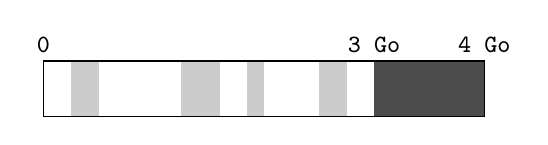
\begin{tikzpicture}
  [scale=0.7
  ,user/.style={fill=black!20}
  ,kernel/.style={fill=black!70}
  ]

  % Memory zone
  %
  % #1 - start
  % #2 - end
  % #3 - color
  \newcommand{\mzone}[3]{
    \path[#3] (#1,0) rectangle (#2,1);
  }

  % Address label
  %
  % #1 - x position
  % #2 - text
  \newcommand{\alabel}[2]{
    \path (#1,1) -- ++(0,0.3) node [pos=1] {\small \tt #2};

  }

  % exec
  \mzone{0.5}{1}{user}

  % lib
  \mzone{2.5}{3.2}{user}

  % stack
  \mzone{3.7}{4}{user}

  % stack
  \mzone{5}{5.5}{user}

  % kernel
  \mzone{6}{8}{kernel}

  % contour
  \draw (0,0) rectangle (8,1);

  \alabel{0}{0}
  \alabel{6}{3 Go}
  \alabel{8}{4 Go}

\end{tikzpicture}

}

\caption{L'espace d'adressage d'un processus. En gris clair, les zones
accessibles à tous les niveaux de privilèges : code du programme, bibliothèques,
tas, pile. En gris foncé, la mémoire du noyau, réservée au mode privilégié.}

\label{fig:memmap}
\end{figure}

\subsection{Appels système}

Les programmes utilisateur s'exécutant en \ring{3}, ils ne peuvent pas
contenir d'instructions privilégiées, et donc ne peuvent pas accéder directement
au matériel (c'était le but !). Pour qu'ils puissent interagir avec le système
(afficher une sortie, écrire sur le disque...), le mécanisme des appels système
est nécessaire. Il s'agit d'une interface de haut niveau entre les \emph{rings}
3 et 0. Du point de vue du programmeur, il s'agit d'un ensemble de fonctions C
``magiques'' qui font appel au système d'exploitation pour effectuer des
opérations.

Prenons le cas de l'appel \texttt{getpid}, qui retourne le numéro de processus
courant. La bibliothèque C fournit une fonction du même nom :

\begin{Verbatim}
pid_t getpid(void);
\end{Verbatim}

A priori, rien de différent d'une fonction implantée directement en C. Par un
processus détaillé ci-après, cette fonction va invoquer la fonction, suivante,
définie dans le noyau (\texttt{kernel/timer.c}) :

\begin{Verbatim}
SYSCALL_DEFINE0(getpid)
{
        return task_tgid_vnr(current);
}
\end{Verbatim}



Le mécanisme de couplage entre ces deux fonctions est le suivant. Une
explication plus détaillé est disponible dans la documentation d'Intel
\cite{intelsys}.

Il y a bien une fonction \texttt{getpid} présente dans la bibliothèque C du
système. C'est la fonction qui est directement appelée par le programme. Cette
fonction commence par placer le numéro de l'appel système (noté
\texttt{\_\_NR\_getpid}, valant 20 ici) dans \eax, puis les arguments éventuels
dans les registres (\ebx, \ecx, \edx, \esi puis \edi). Une interruption
logicielle est ensuite déclenchée (\texttt{int 0x80}) : étant donné la
configuration du processeur, elle sera traitée en \ring{0}, à un point
d'entrée prédéfini (\texttt{arch/x86/kernel/entry\_32.S},
\texttt{ENTRY(system\_call)}).

L'exécution reprend donc en \ring{0}, avec une pile propre au processus.
Les valeurs des registres ont été préservées : elles sont mises sur la pile du
noyau. Le noyau examine le numéro d'appel système (toujours dans \eax) et
appelle la fonction correspondante dans le tableau \texttt{sys\_call\_table} :
les arguments sont en place sur la pile, comme dans le cas d'un appel de
fonction ``classique''. La fonction, nommée \texttt{sys\_getpid}, peut donc être
écrite en C.

Au retour de la fonction, la valeur de retour est placée à la place de \eax là
où les registres ont été sauvegardés sur la pile noyau. L'instruction
\texttt{iret} permet de restaurer les registres et de repasser en mode
utilisateur, juste après l'interruption. La fonction de la bibliothèque C peut
alors retourner au programme appelant.

% vim: spelllang=fr
